%*******************************************************************************
%*********************************** Fifth Chapter *****************************
%*******************************************************************************

\chapter{Density Measurement Induced Dynamics}
% Title of the Fifth Chapter

\ifpdf
    \graphicspath{{Chapter5/Figs/Raster/}{Chapter5/Figs/PDF/}{Chapter5/Figs/}}
\else
    \graphicspath{{Chapter5/Figs/Vector/}{Chapter5/Figs/}}
\fi


\section{Introduction}

In the previous chapter we have introduced a theoretical framework
which will allow us to study measurement backaction using
discontinuous quantum jumps and non-Hermitian evolution due to null
outcomesquantum trajectories. We have also wrapped our quantum gas
model in this formalism by considering ultracold bosons in an optical
lattice coupled to a cavity which collects and enhances light
scattered in one particular direction. One of the most important
conclusions of the previous chapter was that the introduction of
measurement introduces a new energy and time scale into the picture
which competes with the intrinsic dynamics of the bosons.

In this chapter, we investigate the effect of quantum measurement
backaction on the many-body state and dynamics of atoms. In
particular, we will focus on the competition between the backaction
and the the two standard short-range processes, tunnelling and on-site
interactions, in optical lattices. We show that the possibility to
spatially structure the measurement at a microscopic scale comparable
to the lattice period without the need for single site resolution
enables us to engineer efficient competition between the three
processes in order to generate new nontrivial dynamics. However,
unlike tunnelling and on-site interactions our measurement scheme is
global in nature which makes it capable of creating long-range
correlations which enable nonlocal dynamical processes. Furthermore,
global light scattering from multiple lattice sites creates nontrivial
spatially nonlocal coupling to the environment which is impossible to
obtain with local interactions \cite{daley2014, diehl2008,
  syassen2008}. These spatial modes of matter fields can be considered
as designed systems and reservoirs opening the possibility of
controlling dissipations in ultracold atomic systems without resorting
to atom losses and collisions which are difficult to manipulate. Thus
the continuous measurement of the light field introduces a
controllable decoherence channel into the many-body dynamics. Such a
quantum optical approach can broaden the field even further allowing
quantum simulation models unobtainable using classical light and the
design of novel systems beyond condensed matter analogues.

In the weak measurement limit, where the quantum jumps do not occur
frequently compared to the tunnelling rate, this can lead to global
macroscopic oscillations of bosons between odd and even sites. These
oscillations occur coherently across the whole lattice enabled by the
fact that measurement is capable of generating nonlocal spatial
modes. When on-site interactions are included we obtain a system with
three competing energy scales of which two correspond to local
processes and one is global. This complicates the picture
immensely. We show how under certain circumstances interactions
prevent measurement from generating globally coherent dynamics, but on
the other hand when the measurement is strong both processes
collaborate in squeezing the atomic distribution.

On the other end of the spectrum, when measurement is strong we enter
the regime of quantum Zeno dynamics. Frequent measurements can slow
the evolution of a quantum system leading to the quantum Zeno effect
where a quantum state is frozen in its initial configuration
\cite{misra1977, facchi2008}. One can also devise measurements with
multi-dimensional projections which lead to quantum Zeno dynamics
where unitary evolution is uninhibited within this degenerate
subspace, usually called the Zeno subspace \cite{facchi2008,
  raimond2010, raimond2012, signoles2014}. Our flexible setup where global light
scattering can be engineered allows us to suppress or enhance specific
dynamical processes thus realising spatially nonlocal quantum Zeno
dynamics. This unconventional variation occurs when measurement is
near, but not in, its projective limit. The system is still confined
to Zeno subspaces, but intermediate transitions are allowed via
virtual Raman-like processes. We show that this result can, in general
(i.e.~beyond the ultracold gas model), be approximated by a
non-Hermitian Hamiltonian thus extending the notion of quantum Zeno
dynamics into the realm of non-Hermitian quantum mechanics joining the
two paradigms.

\section{Large-Scale Dynamics due to Weak Measurement}

We start by considering the weak measurement limit when photon
scattering does not occur frequently compared to the tunnelling rate
of the atoms, i.e.~$\gamma \ll J$. When the system is probed in this
way, the measurement is unable to project the quantum state of the
bosons to an eigenspace as postulated by the Copenhagen interpretation
of quantum mechanics. The backaction of the photodetections is simply
not strong or frequent enough to confine the atoms. However, instead
of confining the evolution of the quantum state, it has been shown in
Refs. \cite{mazzucchi2016, mazzucchi2016njp} that the measurement
leads to coherent global oscillations between the modes generated by
the spatial profile of the light field which we have seen in section
\ref{sec:modes}. Fig. \ref{fig:oscillations} illustrates the atom
number distributions in the odd sites for $Z = 2$ and one of the three
modes for $Z = 3$. These oscillations correspond to atoms flowing from
one mode to another. We only observe a small number of well defined
components which means that this flow happens in phase, all the atoms
are tunnelling between the modes together in unison. Furthermore, this
exchange of population is macroscopic in scale. The trajectories reach
a state where the maximum displacement point corresponds to all the
atoms being entirely within a single mode. Finally, we note that these
oscillating distributions are squeezed by the measurement and the
individual components have a width smaller than the initial state. By
contrast, in the absence of the external influence of measurement
these distributions would spread out significantly and the center of
the broad distribution would oscillate with an amplitude comparable to
the initial imbalance, i.e.~small oscillations for a small initial
imbalance.

\begin{figure}[htbp!]
  \centering
  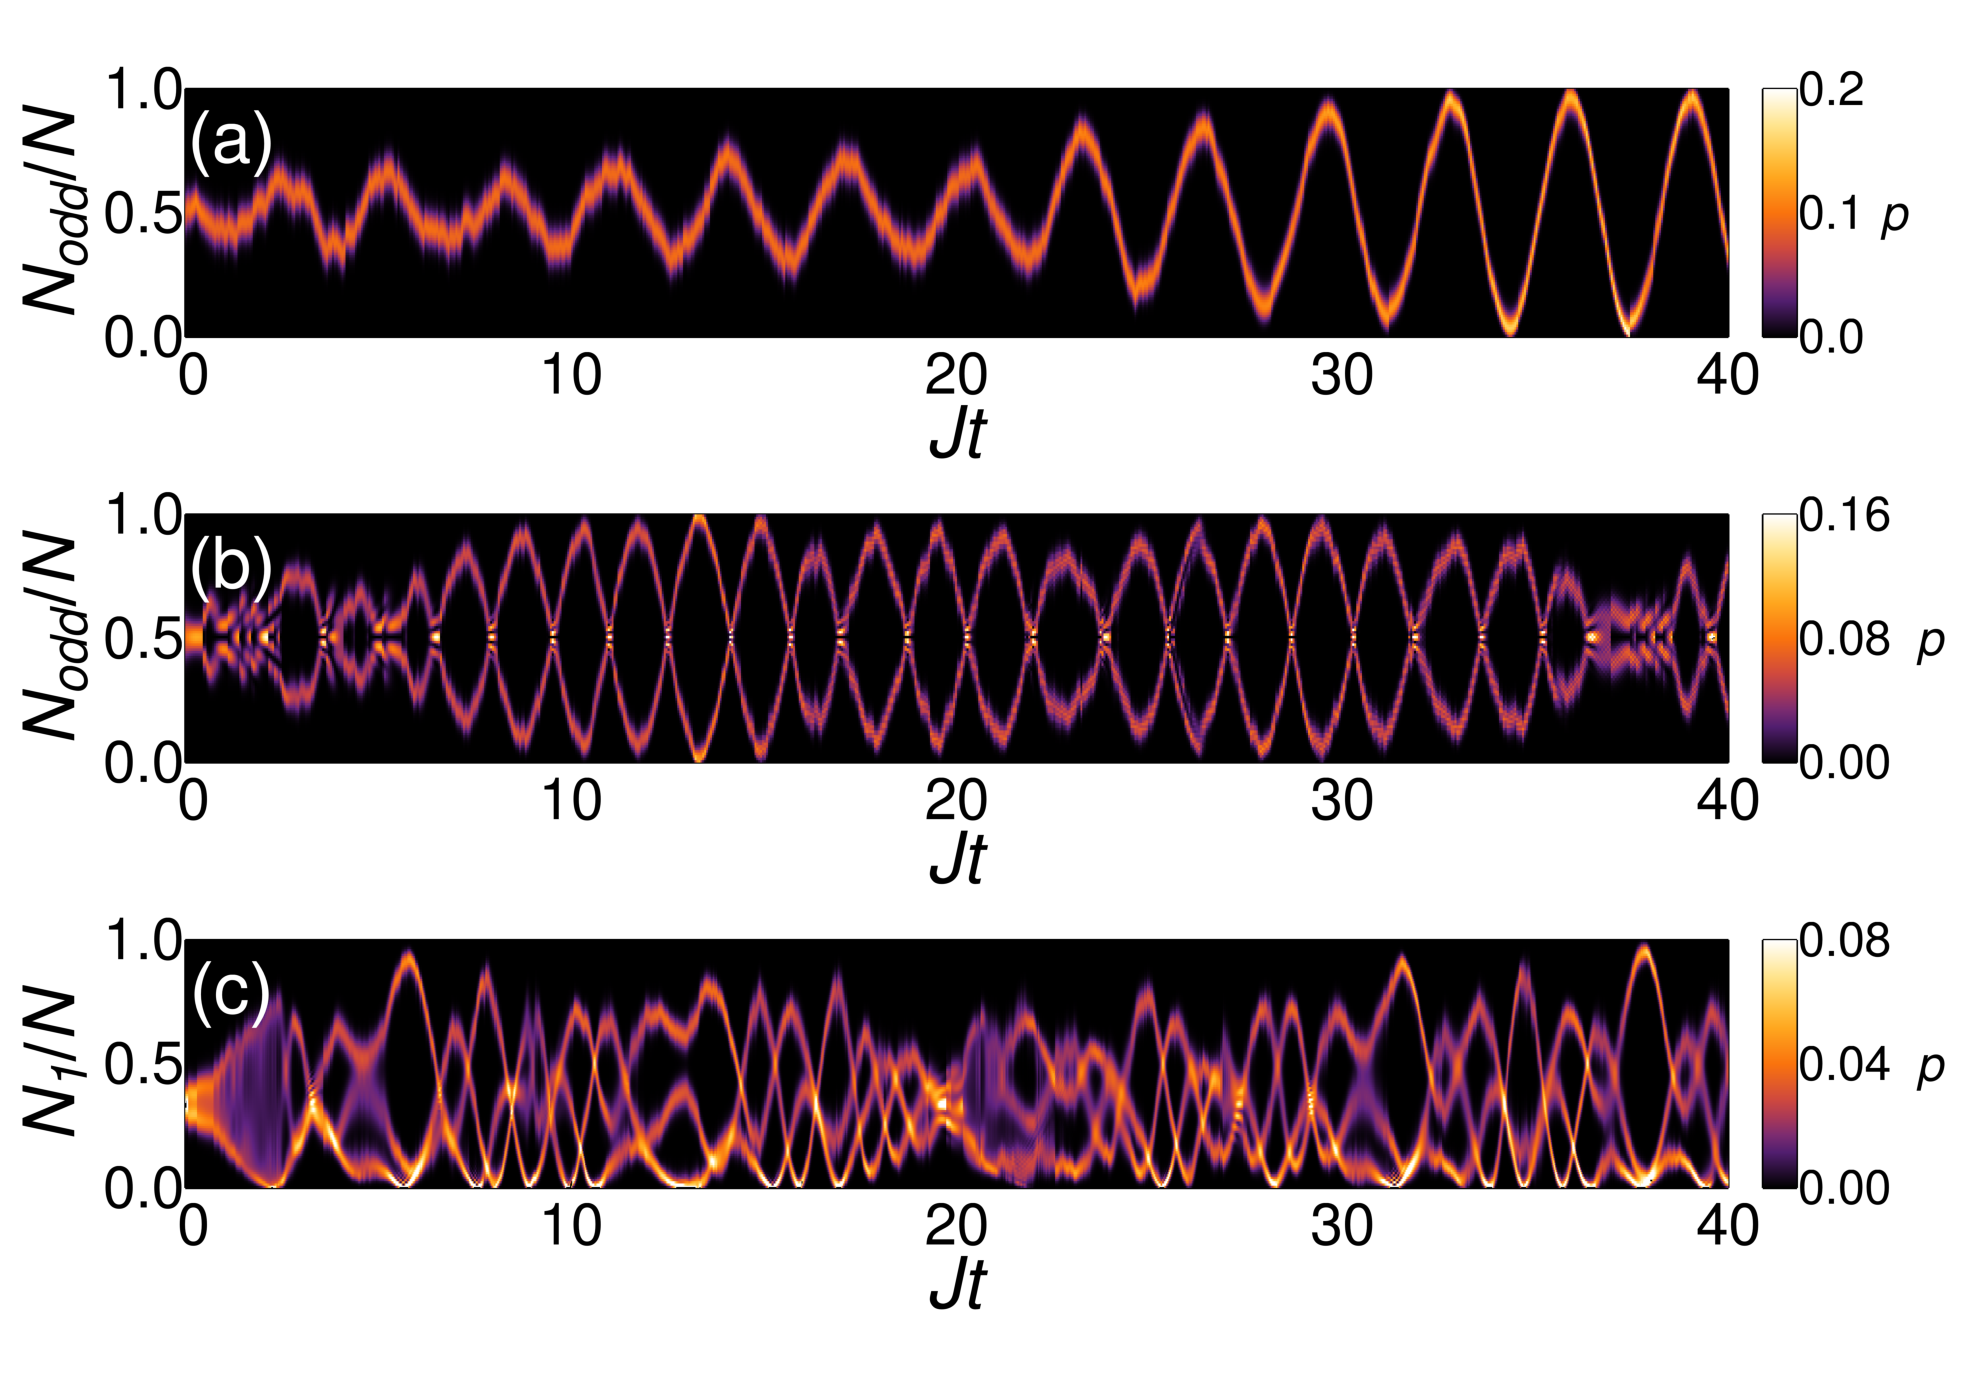
\includegraphics[width=\textwidth]{Oscillations}
  \caption[Macroscopic Oscillations due to Weak Measurement]{Large
    oscillations between the measurement-induced spatial modes
    resulting from the competition between tunnelling and weak
    measurement induced backaction. The plots show the atom number
    distributions $p(N_l)$ in one of the modes in individual quantum
    trajectories. These dstributions show various numbers of
    well-squeezed components reflecting the creation of macroscopic
    superposition states depending on the measurement
    configuration. $U/J = 0$, $\gamma/J = 0.01$, $M=N$, initial
    states: bosonic superfluid. (a) Measurement of the atom number at
    odd sites $\hat{N}_\mathrm{odd}$ creates one strongly oscillating
    component in $p(N_\mathrm{odd})$ ($N = 100$ bosons, $J_{j,j} = 1$
    if $j$ is odd and 0 otherwise). (b) Measurement of
    $(\hat{N}_\mathrm{odd} - \hat{N}_\mathrm{even})^2$ introduces
    $Z = 2$ modes and preserves the superposition of positive and
    negative atom number differences in $p(N_\mathrm{odd})$ ($N = 100$
    bosons, $J_{j,j} = (-1)^{j+1}$). (c) Measurement for $Z = 3$ modes
    preserves three components in $p(N_1)$ ($N = 108$ bosons,
    $J_{j,j} = e^{i 2 \pi j / 3}$).}
  \label{fig:oscillations}
\end{figure}

In Figs. \ref{fig:oscillations}(b,c) we also see that the system is
composed of multiple components. This depends on the quantity that is
being measured and it is a consequence of the fact that the detected
light intensity $\ad_1 \a_1$ is not sensitive to the light phase. The
measurement will not distinguish between permutations of mode
occupations that scatter light with the same intensity, but with a
different phase. For example, when measuring
$\hat{D} = \hat{N}_\mathrm{odd} - \hat{N}_\mathrm{even}$, the light
intensity will be proportional to
$\hat{D}^\dagger \hat{D} = (\hat{N}_\mathrm{odd} -
\hat{N}_\mathrm{even})^2$ and thus it cannot distinguish between a
positive and negative imbalance leading to the two components seen in
Fig. \ref{fig:oscillations}. More generally, the number of components
of the atomic state, i.e.~the degeneracy of $\ad_1 \a_1$, can be
computed from the eigenvalues of Eq. \eqref{eq:Zmodes},
\begin{equation}
  \hat{D} = \sum_l^Z \exp\left[-i 2 \pi l R / Z \right] \hat{N}_l.
\end{equation}
Each eigenvalue can be represented as the sum of the individual terms
in teh above sum which are vectors on the complex plane with phases
that are integer multiples of $2 \pi / Z$: $N_1 e^{-i 2 \pi R / Z}$,
$N_2 e^{-i 4 \pi R / Z}$, ..., $N_Z$. Since the set of possible sums
of these vectors is invariant under rotations by $2 \pi l R / Z$,
$l \in \mathbb{Z}$, and reflection in the real axis, the state of the
system is 2-fold degenerate for $Z = 2$ (reflections leave $Z = 2$
unchanged) and $2Z$-fold degenerate for $Z >
2$. Fig. \ref{fig:oscillations} shows the three mode case, where there
are in fact $6$ components ($2Z = 6$), but in this case they all occur
in pairs resulting in only three visible components.

We will now limit ourselves to a specific illumination pattern with
$\hat{D} = \hat{N}_\mathrm{odd}$ as this leads to the simplest
multimode dynamics with $Z = 2$ and only a single component as seen in
Fig. \ref{fig:oscillations}a, i.e.~no multiple peaks like in
Figs. \ref{fig:oscillations}(b,c). This pattern can be obtained by
crossing two beams such that their projections on the lattice are
identical and the even sites are positioned at their nodes. However,
even though this is the simplest possible case and we are only dealing
with non-interacting atoms solving the full dynamics of the
Bose-Hubbard Hamiltonian combined with measurement is nontrivial. The
backaction introduces a highly nonlinear global term. However, it has
been shown in Ref. \cite{mazzucchi2016njp} that the non-interacting
dynamics with quantum measurement backaction for $Z$-modes reduce to
an effective Bose-Hubbard Hamiltonian with $Z$-sites provided the
initial state is a superfluid. In this simplified model the $N_j$
atoms in the $j$-th site correspond to a superfluid of $N_j$ atoms
within a single spatial mode as defined in section
\ref{sec:modes}. Therefore, we now proceed to study the dynamics for
$\hat{D} = \hat{N}_\mathrm{odd}$ using this reduced effective
double-well model.

The atomic state can be written as
\begin{equation}
  \label{eq:discretepsi}
  | \psi \rangle = \sum_l^N q_l |l, N - l \rangle,
\end{equation}
where the ket $| l, N - l \rangle$, represents a superfluid with $l$
atoms in the odd sites and $N-l$ atoms in the even sites. The
non-Hermitian Hamiltonian describing the time evolution in between the
jumps is given by
\begin{equation}
  \label{eq:doublewell}
  \hat{H} = -J^\mathrm{cl} \left( \bd_o b_e + b_o \bd_e \right) - i
  \gamma \n_o^2
\end{equation}
and the quantum jump operator which is applied at each photodetection
is $\c = \sqrt{2 \kappa} C \n_o$. $b_o$ ($\bd_o$) is the annihilation
(creation) operator in the left site of the effective double-well
corresponding to the superfluid at odd sites of the physical
lattice. $b_e$ ($\bd_e$) is defined similarly, but for the right site
and the superfluid at even sites of the physical lattice.
$\n_o = \bd_o b_o$ is the atom number operator in the left site.

Even though Eq. \eqref{eq:doublewell} is relatively simple as it it is
only a non-interacting two-site model, the non-Hermitian term
complicates the situation making the system difficult to
solve. However, a semiclassical approach to boson dynamics in a
double-well in the limit of many atoms $N \gg 1$ has been developed in
Ref. \cite{juliadiaz2012}. It was originally formulated to treat
squeezing in a weakly interacting bosonic gas, but it can easily be
applied to our system as well. In the limit of large atom number, the
wavefunction in Eq. \eqref{eq:discretepsi} can be described using
continuous variables by defining $\psi (x = l / N) = \sqrt{N}
q_l$. Note that this requires the coefficients $q_l$ to vary smoothly
which is the case for a superfluid state. We now rescale the
Hamiltonian in Eq. \eqref{eq:doublewell} to be dimensionless by
dividing by $NJ^\mathrm{cl}$ and define the relative population
imbalance between the two wells $z = 2x - 1$. Finally, by taking the
expectation value of the Hamiltonian and looking for the stationary
points of
$\langle \psi | \hat{H} | \psi \rangle - E \langle \psi | \psi
\rangle$ we obtain the semiclassical Schr\"{o}dinger equation
\begin{equation}
  \label{eq:semicl}
  i h \partial_t \psi(z, t) = \mathcal{H} \psi(z, t),
\end{equation}
\begin{equation}
  \label{eq:semiH}
  \mathcal{H} \approx -2 h^2 \partial^2_z \psi(z, t) + \left[
    \frac{\omega^2 z^2} {8} - \frac{i \Gamma} {4} \left( z + 1
    \right)^2 \right] \psi(z, t),
\end{equation}
where $\Gamma = N \kappa |C|^2 / J$, $h = 1/N$,
$\omega = 2 \sqrt{1 + \Lambda - h}$, and
$\Lambda = NU / (2J^\mathrm{cl})$. The full derivation is not
straightforward, but the introduction of the non-Hermitian term
requires only a minor modification to the original formalism presented
in detail in Ref. \cite{juliadiaz2012} so we have omitted it here. We
will also be considering $U = 0$ as the effective model is only valid
in this limit, thus $\Lambda = 0$. However, this model is valid for an
actual physical double-well setup in which case interacting bosons can
also be considered. The equation is defined on the interval
$z \in [-1, 1]$, but $z \ll 1$ has been assumed in order to simplify
the kinetic term and approximate the potential as parabolic. This does
mean that this approximation is not valid for the maximum amplitude
oscillations seen in Fig. \ref{fig:oscillations}a, but since they
already appear early on in the trajectory we are able to obtain a
valid analytic description of the oscillations and their growth.

A superfluid state in our continuous variable approximation
corresponds to a Gaussian wavefunction $\psi$. Furthermore, since the
potential is parabolic, even with the inclusion of the non-Hermitian
term, it will remain Gaussian during subsequent time
evolution. Therefore, we will use a very general Gaussian wavefunction
of the form
\begin{equation}
  \label{eq:ansatz}
  \psi(z, t) = \frac{1}{\pi b^2}\exp\left[ i \epsilon 
  - \frac{(z - z_0)^2} {2 b^2} + \frac{i \phi (z - z_\phi)^2} {2 b^2} \right]
\end{equation}
as our ansatz to Eq. \eqref{eq:semicl}. The parameters $b$, $\phi$,
$z_0$, and $z_\phi$ are real-valued functions of time whereas
$\epsilon$ is a complex-valued function of time. Physically, the value
$b^2$ denotes the width, $z_0$ the position of the center, $\phi$ and
$z_\phi$ contain the local phase information, and $\epsilon$ only
affects the global phase and norm of the Gaussian wave packet.

The non-Hermitian Hamiltonian and an ansatz are not enough to describe
the full dynamics due to measurement. We also need to know the effect
of each quantum jump. Within the continuous variable approximation,
our quantum jump become $\c \propto 1 + z$. We neglect the constant
prefactors, because the wavefunction is normalised after a quantum
jump. Expanding around the peak of the Gaussian ansatz we get
\begin{equation}
  1 + z \approx \exp \left[ \ln (1 + z_0) + \frac{z - z_0}{1 + z_0} -
    \frac{(z - z_0)^2}{2 (1 + z_0)^2} \right].
\end{equation}
Multiplying the wavefunction in Eq. \eqref{eq:ansatz} with the jump
operator above yields a Gaussian wavefunction as well, but the
parameters change discontinuously according to
\begin{align}
  \label{eq:jumpb2}
  b^2 & \rightarrow \frac{ b^2 (1 + z_0)^2 } { (1 + z_0)^2 + b^2 }, \\
  \phi & \rightarrow \frac{ \phi (1 + z_0)^2 } { (1 + z_0)^2 + b^2 }, \\
  \label{eq:jumpz0}
  z_0 & \rightarrow z_0 + \frac{ b^2 (1 + z_0) } { (1 + z_0)^2 + b^2}, \\
  z_\phi & \rightarrow z_\phi, \\
  \epsilon & \rightarrow \epsilon.
\end{align}
The fact that the wavefunction remains Gaussian after a photodetection
is a huge advantage, because it means that the combined time evolution
of the system can be described with a single Gaussian ansatz in
Eq. \eqref{eq:ansatz} subject to non-Hermitian time evolution
according to Eq. \eqref{eq:semicl} with discontinous changes to the
parameter values at each quantum jump.

Having identified an appropriate ansatz and the effect of quantum
jumps we proceed with solving the dynamics of wavefunction in between
the photodetecions. The initial values of the parameters for a
superfluid state of $N$ atoms across the whole lattice are $b^2 = 2h$,
$\phi =0$, $a_0 = 0$, $a_\phi = 0$, $\epsilon = 0$. However, we use
the most general initial conditions at time $t = t_0$ which we denote
by $b(t_0) = b_0$, $\phi(t_0) = \phi_0$, $z_0(t_0) = a_0$,
$z_\phi(t_0) = a_\phi$, and $\epsilon(t_0) = \epsilon_0$. The reason
for keeping them as general as possible is that after every quantum
jump the system changes discontinuously. The subsequent time evolution
is obtained by solving the Schr\"{o}dinger equation with the post-jump
paramater values as the new initial conditions.

By plugging the ansatz in Eq. \eqref{eq:ansatz} into the
Schr\"{o}dinger equation in Eq. \eqref{eq:semicl} we obtain three
differential equations
\begin{equation}
  \label{eq:p}
  -2 h^2 p^2 + \left( \frac{ \omega^2 } { 8 } - \frac{ i \Gamma } { 4
    } \right) + \frac{ i h } { 2 } \frac{ \mathrm{d} p } { \mathrm{d}
    t } = 0,
\end{equation}
\begin{equation}
  \label{eq:pq}
  4 h^2 p q - \frac{ i \Gamma } { 2 } - i h \frac{ \mathrm{d} q } {
    \mathrm{d} t } = 0
\end{equation}
\begin{equation}
  \label{eq:pqr}
  -2 h^2 (q^2 - p) - \frac{ i \Gamma } { 4 } - i h \left( \frac{ 1 } {
      4 x } \frac{ \mathrm{d} x } {\mathrm{d} t } + i \frac{
      \mathrm{d} \epsilon } { \mathrm{d} t } - \frac{1}{2} \frac{
      \mathrm{d} r } { \mathrm{d} t } \right) = 0,
\end{equation}
where $x = 1/b^2$, $p = (1 - i \phi)/b^2$,
$q = (z_0 - i \phi z_\phi)/b^2$, and
$r = (z_0^2 - \phi z_\phi^2)/b^2$. The corresponding initial
conditions are $x(t_0) = x_0 = 1/b_0^2$,
$p(t_0) = p_0 = (1 - i \phi_0)/b_0^2$,
$q(t_0) = q_0 = (a_0 - \phi_0 a_\phi)/b_0^2$, and
$r(t_0) = r_0 = (a_0^2 - \phi_0 a_\phi^2)/b_0^2$. The original
parameters can be extracted from these auxiliary variables by
$b^2 = 1 / \Re \{ p \}$, $\phi = - \Im \{ p \} / \Re \{ p \}$,
$z_0 = \Re \{ q \} / \Re \{ p \}$,
$z_\phi = \Im \{ q \} / \Im \{ p \}$, and $\epsilon$ appears
explicitly in the equations above.

First, it is worth noting that all parameters of interest can be
extracted from $p(t)$ and $q(t)$ alone. We are not interested in
$\epsilon$ as it is only related to the global phase and the norm of
the wavefunction and it contains little physical
information. Furthermore, an interesting and incredibly convenient
feature of these equations is that the Eq. \eqref{eq:p} is a function
of $p(t)$ alone and Eq. \eqref{eq:pq} is a function of $p(t)$ and
$q(t)$ only. Therefore, we only need to solve first two equations and
we can neglect Eq. \eqref{eq:pqr}. However, in order to actually
perform Monte-Carlo simulations of quantum trajectories
Eq. \eqref{eq:pqr} would need to be solved in order to obtain correct
jump statistics.

We start with Eq. \eqref{eq:p} and we note it can be rearranged into
the form
\begin{equation}
  \frac{ \mathrm{d} p } { (\zeta \omega / 4 h)^2 - p^2 } = i 4 h
  \mathrm{d} t,
\end{equation}
where $\zeta^2 = (\alpha - i \beta)^2 = 1 - i 2 \Gamma / \omega^2$, and
\begin{equation}
  \alpha = \sqrt{ \frac{1}{2} + \frac{1}{2} \sqrt{1 + \frac{ 4\Gamma^2
      }{ \omega^4 }}},
\end{equation}
\begin{equation}
  \beta = -\sqrt{ -\frac{1}{2} + \frac{1}{2} \sqrt{1 + \frac{ 4\Gamma^2
      }{ \omega^4 }}}.
\end{equation}
This is a standard integral\footnotemark and thus yields
\begin{equation}
  \label{eq:psol}
  p(t) = \frac{ \zeta \omega } { 4 h } 
  \frac{ ( \zeta \omega + 4 h p_0 )e^{i \zeta \omega t} - ( \zeta
    \omega - 4 h p_0 ) e^{-i \zeta \omega t} }
  { ( \zeta \omega + 4 h p_0 )e^{i \zeta \omega t} + ( \zeta \omega
    - 4 h p_0 ) e^{-i \zeta \omega t} }.
\end{equation}

\footnotetext{ \[ \int \frac{\mathrm{d} x}{a^2 - x^2} = \frac{1}{2a}
    \ln \left( \frac{a+x}{a-x} \right) + \mathrm{const.} 
    \quad\quad\quad\quad\quad\quad\quad\quad\quad\quad\quad\quad\quad\quad\quad
    \quad\quad\quad\quad\quad\] }

Having found an expression for $p(t)$ we can now solve
Eq. \eqref{eq:pq} for $q(t)$. To do that we first define the
integrating factor
\begin{equation}
  I(t) = \exp \left[ i 4 h \int p \mathrm{d} t \right] = ( \zeta
  \omega + 4 h p_0 )e^{i \zeta \omega t} + ( \zeta \omega - 4 h p_0 )
  e^{-i \zeta \omega t},
\end{equation}
which lets us rewrite Eq. \eqref{eq:pq} as
\begin{equation}
  \label{eq:Iq}
  \frac{\mathrm{d}} {\mathrm{d} t}(Iq) = - \frac{\Gamma}{2 h} I.
\end{equation}
%Upon integrating the equation above we obtain
%\begin{equation}
%  \label{eq:Iq}
%  Iq = - \frac{ \Gamma } {2 h} \int I \mathrm{d} t.
%\end{equation}
Upon integrating and the substitution of the explicit form of the
integration factor into this equation we obtain the solution
\begin{equation}
  \label{eq:qsol}
  q(t) = \frac{1}{2 h \zeta \omega} 
  \frac{4 h \zeta^2 \omega^2 q_0 - i 8 h \Gamma p_0
    + i \Gamma [( \zeta \omega + 4 h p_0 )e^{i \zeta \omega t} - 
    ( \zeta \omega - 4 h p_0 )e^{-i \zeta \omega t}]}
  { ( \zeta \omega + 4 h p_0 )e^{i \zeta \omega t} + 
    ( \zeta \omega - 4 h p_0 )e^{-i \zeta \omega t}}.
\end{equation}

The solutions we have obtained to $p(t)$ in Eq. \eqref{eq:psol} and
$q(t)$ in Eq. \eqref{eq:qsol} are sufficient to completely describe
the physics of the system. Unfortunately, these expressions are fairly
complex and it is difficult to extract the physically meaningful
parameters in a form that is easy to analyse. Therefore, we instead
consider the case when $\Gamma = 0$, but we do not neglect the effect
of quantum jumps. It may seem counter-intuitive to neglect the term
that appears due to measurement, but we are considering the weak
measurement regime where $\gamma \ll J^\mathrm{cl}$ and thus the
dynamics between the quantum jumps are actually dominated by the
tunnelling of atoms rather than the null outcomes. Furthermore, the
effect of the quantum jump is independent of the value of $\Gamma$
($\Gamma$ only determined their frequency). However, this is only true
at times shorter than the average time between two consecutive quantum
jumps. Therefore, this approach will not yield valid answers on the
time scale of a whole quantum trajectory, but it will give good
insight into the dynamics immediately after a quantum jump. The
solutions for $\Gamma = 0$ are
\begin{equation}
b^2(t) = \frac{b_0^2}{2} \left[ \left(1 + \frac{16 h^2 (1 + \phi_0^2)}
    {b_0^4 \omega^2} \right) + \left(1 - \frac{16 h^2 (1 + \phi_0^2)}
    {b_0^4 \omega^2} \right) \cos (2 \omega t) + \frac{8 h \phi_0}{b_0^2
    \omega} \sin(2 \omega t) \right],
\end{equation}
\begin{equation}
  \phi(t) = \frac{b_0^2 \omega} {8 h} \left[ \left( \frac{16 h^2 (1 + \phi_0^2)}
      {b_0^4 \omega^2} - 1 \right) \sin (2 \omega t) + \frac{8 h
      \phi_0} {b_0^2 \omega} \cos (2 \omega t) \right],
\end{equation}
\begin{equation}
  z_0(t) = a_0 \cos(\omega t) + \frac{4 h \phi_0} {b_0^2 \omega} (a_0 -
  a_\phi) \sin (\omega t),
\end{equation}
\begin{equation}
  \phi(t) z_\phi(t) = \phi_0 a_\phi \cos (\omega t)  + \frac{4 h}
  {b_0^2 \omega} (a_0 - \phi_0^2 a_\phi) \sin( \omega t).
\end{equation}
First, these equations show that all quantities oscillate with a
frequency $\omega$ or $2 \omega$. We are in particular interested in
the quantity $z_0(t)$ as it represents the position of the peak of the
wavefunction and we see that it oscillates with an amplitude
$\sqrt{a_0^2 + 16 h^2 \phi_0^2 (a_0 - a_\phi)^2 / (b_0^4
  \omega^2)}$. Thus we have obtained a solution that clearly shows
oscillations of a single Gaussian wave packet. The fact that this
appears even when $\Gamma = 0$ shows that the oscillations are a
property of the Bose-Hubbard model itself. However, they also depend
on the initial conditions and for these oscillations to occur, $a_0$
and $a_\phi$ cannot be zero, but this is exactly the case for an
initial superfluid state. We have seen in Eq. \eqref{eq:jumpz0} that
the effect of a photodetection is to displace the wavepacket by
approximately $b^2$, i.e.~the width of the Gaussian, in the direction
of the positive $z$-axis. Therefore, even though the can oscillate in
the absence of measurement it is the quantum jumps that are the
driving force behind this phenomenon. Furthermore, these oscillations
grow because the quantum jumps occur at an average instantaneous rate
proportional to $\langle \cd \c \rangle (t)$ which itself is
proportional to $(1+z)^2$. This means they are most likely to occur at
the point of maximum displacement in the positive $z$ direction at
which point a quantum jump provides positive feedback and further
increases the amplitude of the wavefunction leading to the growth seen
in Fig. \ref{fig:oscillations}a. The oscillations themselves are
essentially due to the natural dynamics of coherently displaced atoms
in a lattice , but it is the measurement that causes the initial and
more importantly coherent displacement and the positive feedback drive
which causes the oscillations to continuously grow.

We have now seen the effect of the quantum jumps and how that leads to
oscillations between odd and even sites in a lattice. However, we have
neglected the effect of null outcomes on the dynamics. Even though it
is small, it will not be negligible on the time scale of a quantum
trajectory with multiple jumps. First, we note that all the
oscillatory terms $p(t)$ and $q(t)$ actually appear as
$\zeta \omega = (\alpha - i \beta) \omega$. Therefore, we can see that
the null outcomes lead to two effects: an increase in the oscillation
frequency by a factor of $\alpha$ to $\alpha \omega$ and a damping
term with a time scale $1/(\beta \omega)$. For weak measurement, both
$\alpha$ and $\beta$ will be close to $1$ so the effects are not
visible on short time scales. Instead, we look at the long time
limit. Unfortunately, since all the quantities are oscillatory a
stationary long time limit does not exist especially since the quantum
jumps provide a driving force. However, the width of the Gaussian,
$b^2$, is unique in that it doesn't oscillate around $b^2 =
0$. Furthermore, from Eq. \eqref{eq:jumpb2} we see that even though it
will decrease discontinuously at every jump, this effect is fairly
small since $b^2 \ll 1$ generally. Therefore, we expect $b^2$ to
oscillate, but with an amplitude that decreases approximately
monotonically with time due to quantum jumps and the
$1/(\beta \omega)$ decay terms, because unlike for $z_0$ the quantum
jumps do not cause further displacement in this quantity. Thus,
neglecting the effect of quantum jumps and taking the long time limit
yields
\begin{equation}
  \label{eq:b2}
  b^2(t \rightarrow \infty) = \frac{4 h} {\gamma \omega} \approx
  b^2_\mathrm{SF} \left( 1 - \frac{\Gamma^2}{32} \right),
\end{equation}
where the approximation on the right-hand side follows from the fact
that $\omega \approx 2$ since we are considering the $N \gg 1$ limit,
and because we are considering the weak measurement limit
$\Gamma^2 / \omega^4 \ll 1$. $b^2_\mathrm{SF} = 2h$ denotes the width
of the initial superfluid state. This result is interesting, because
it shows that the width of the Gaussian distribution is squeezed as
compared with its initial state which is exactly what we see in
Fig. \ref{fig:oscillations}a. However, if we substitute the parameter
values used in that trajectory we only get a reduction in width by
about $3\%$, but the maximum amplitude oscillations in look like they
have a significantly smaller width than the initial distribution. This
discrepancy is due to the fact that the continuous variable
approximation is only valid for $z \ll 1$ and thus it cannot explain
the final behaviour of the system. Furthermore, it has been shown that
the width of the distribution $b^2$ does not actually shrink to a
constant value, but rather it keeps oscillating around the value given
in Eq. \eqref{eq:b2} \cite{mazzucchi2016njp}. However, what we do see
is that during the early stages of the trajectory, which are well
described by this model, is that the width does in fact stay roughly
constant. It is only in the later stages when the oscillations reach
maximal amplitude that the width becomes visibly reduced.

\section{Three-Way Competition}

Now it is time to turn on the inter-atomic interactions,
$U/J^\mathrm{cl} \ne 0$. As a result the atomic dynamics will change
as the measurement now competes with both the tunnelling and the
on-site interactions. A common approach to study such open systems is
to map a dissipative phase diagram by finding the steady state of the
master equation for a range of parameter values
\cite{kessler2012}. However, here we adopt a quantum optical approach
in which we focus on the conditional dynamics of a single quantum
trajectory as this corresponds to a single realisation of an
experiment. The resulting evolution does not necessarily reach a
steady state and usually occurs far from the ground state of the
system.

A key feature of the quantum trajectory approach is that each
trajectory evolves differently as it is conditioned on the
photodetection times which are determined stochastically. Furthermore,
even states in the same measurement subspace, i.e.~indistinguishable
to the measurement , can have minimal overlap. This is in contrast to
the unconditioned solutions obtained with the master equation which
only yields a single outcome that is an average taken over all
possible outcomes. However, this makes it difficult to study the
three-way competition in some meaningful way across the whole
parameter range.

Ultimately, regardless of its strength measurement always tries to
project the quantum state onto one of its eigenstates (or eigenspaces
if there are degeneracies). If the probe is strong enough this will
succeed, but we have seen in the previous section that when this is
not the case, measurement leads to new dynamical phenomena. However,
despite this vast difference in behaviour, there is a single quantity
that lets us determine the degree of success of the projection, namely
the fluctuations, $\sigma_D^2$ (or equivalently the standard
deviation, $\sigma_D$), of the observable that is being measured,
$\hat{D}$. For a perfect projection this value is exactly zero,
because the system at that point is in the corresponding
eigenstate. When the system is unable to project the state into such a
state, the variance will be non-zero. However, the smaller its value
is the closer it is to being in such an eigenstate and on the other
hand a large variance means that the internal processes dominate the
competition. Finally, this quantity is perfect to study quantum
trajectories, because its value in the long-time limit it is only a
function of $\gamma$, $J$, and $U$. It does not depend on the explicit
history of photodetections. Fig. \ref{fig:squeezing} shows a plot of
this quantity for $\hat{D} = \hat{N}_\mathrm{odd}$ averaged over
multiple trajectories, $\langle \sigma^2_D \rangle_\mathrm{traj}$, as
a function of $\gamma/J$ and $U/J$ for a lattice of six atoms on six
sites (we cannot use the effective double-well model, because
$U \ne 0$). We use a ground state of for the corresponding $U$ and $J$
values as this provides a realistic starting point and a reference for
comparing the measurement induced dynamics. We will also consider only
$\hat{D} = \hat{N}_\mathrm{odd}$ unless stated otherwise.

\begin{figure}[htbp!]
  \centering
  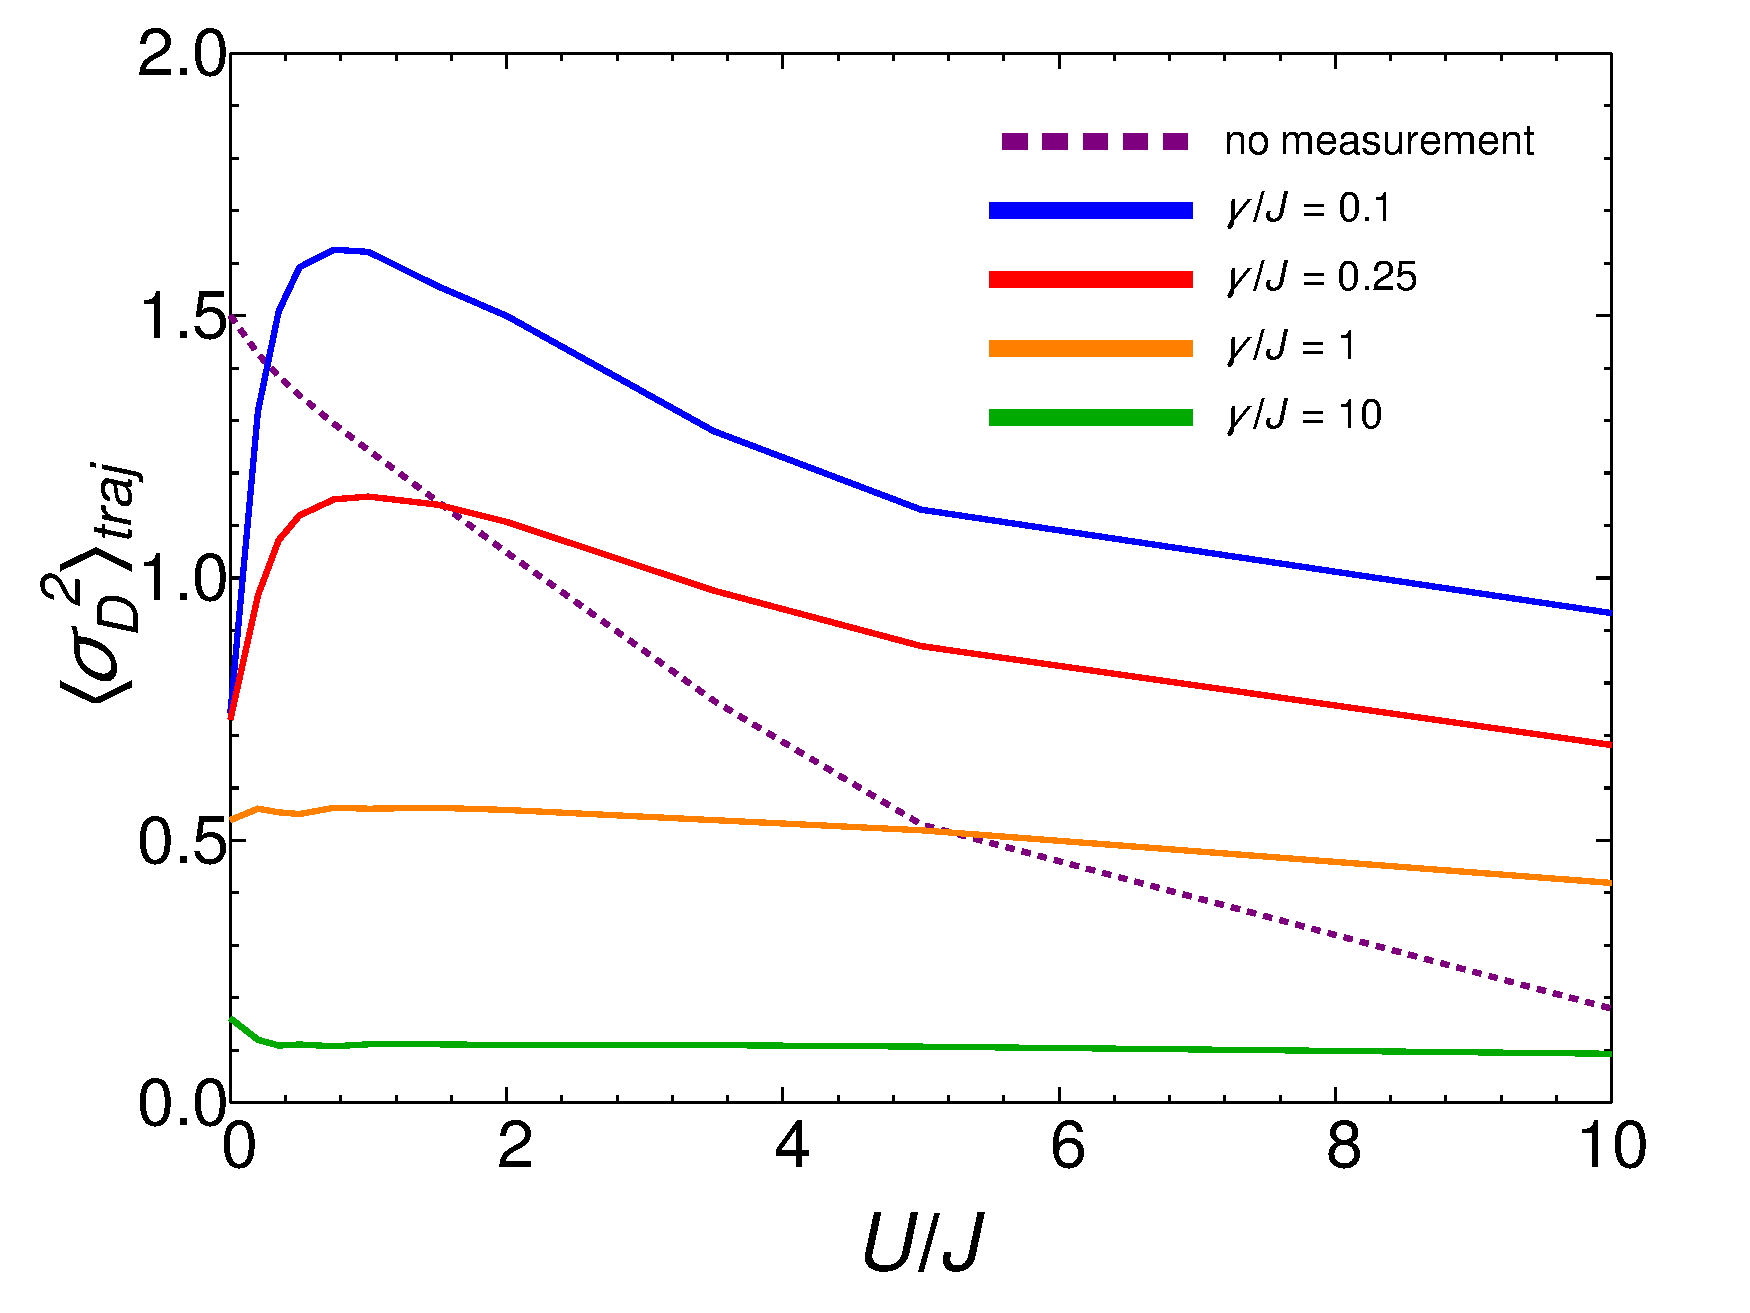
\includegraphics[width=\textwidth]{Squeezing}
  \caption[Squeezing in the presence of Interactions]{Atom number
    fluctuations at odd sites for for $N = 6$ atoms at $M = 6$ sites
    subject to a $\hat{D} = \hat{N}_\mathrm{odd}$ measurement
    demonstrating the competition of global measurement with local
    interactions and tunnelling. Number variances are averaged over
    100 trajectories. Error bars are too small to be shown
    ($\sim 1\%$) which emphasizes the universal nature of the
    squeezing. The initial state used was the ground state for the
    corresponding $U$ and $J$ value. The fluctuations in the ground
    state without measurement decrease as $U / J$ increases,
    reflecting the transition between the supefluid and Mott insulator
    phases. For weak measurement values
    $\langle \sigma^2_D \rangle_\mathrm{traj}$ is squeezed below the
    ground state value for $U = 0$, but it subsequently increases and
    reaches its maximum as the atom repulsion prevents the
    accumulation of atoms prohibiting coherent oscillations thus
    making the squeezing less effective. In the strongly interacting
    limit, the Mott insulator state is destroyed and the fluctuations
    are larger than in the ground state as weak measurement isn't
    strong enough to project into a state with smaller fluctuations
    than the ground state.}
  \label{fig:squeezing}
\end{figure}

First, it is important to note that even though we are dealing with an
average over many trajectories this information cannot be extracted
from a master equation solution. This is because the variance of
$\hat{D}$ as calculated from the density matrix would be dominated by
the uncertainty of the final state. In other words, the fact that the
final value of $\hat{D}$ is undetermined is included in this average
and thus the fluctuations obtained this way are representative of the
variance in the final outcome rather than the squeezing of an
individual conditioned trajectory. This highlights the fact that
interesting physics happens on a single trajectory level which would
be lost if we studied an ensemble average.

\begin{figure}[htbp!]
  \centering
  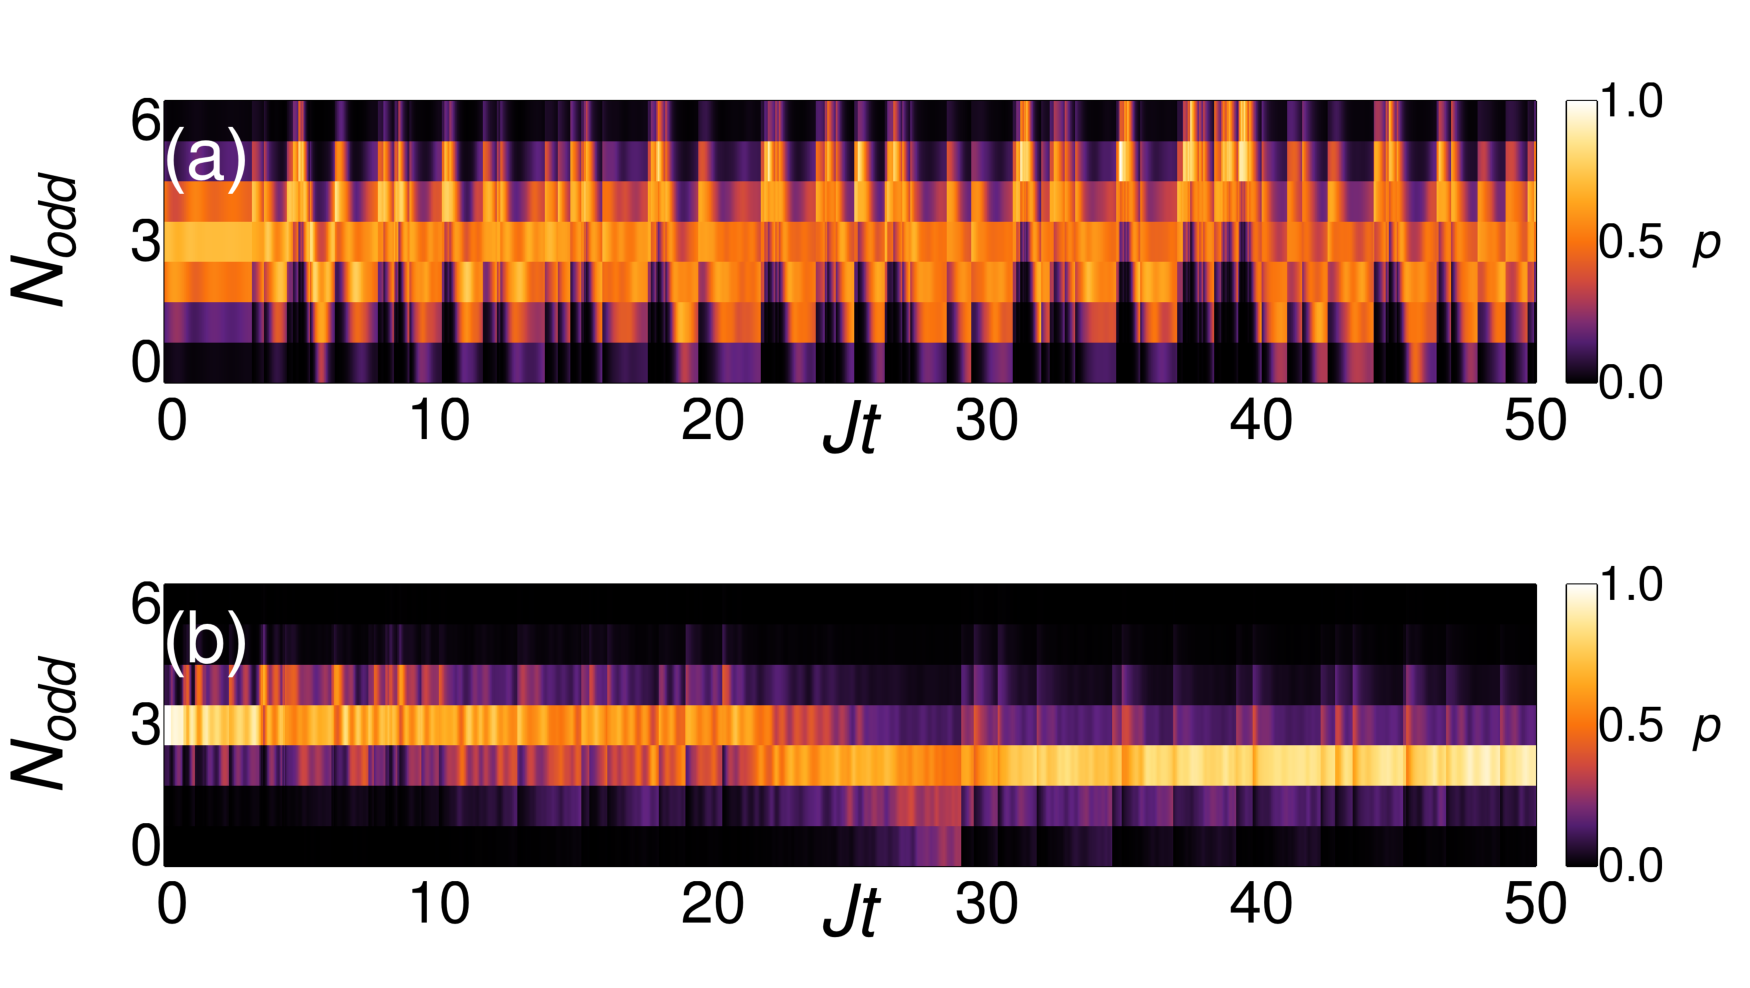
\includegraphics[width=\textwidth]{panel_U}
  \caption[Trajectories in the presence of Interactions]{Conditional
    dynamics of the atom-number distributions at odd sites
    illustrating competition of the global measurement with local
    interactions and tunnelling. The plots are for single quantum
    trajectores starting from the ground state for $N = 6$ atoms on
    $M = 6$ sites with $\hat{D} = \hat{N}_\mathrm{odd}$,
    $\gamma/J = 0.1$. (a) Weakly interacting bosons $U/J = 1$: the
    on-site repulsion prevents the formation of well-defined
    oscillation in the population of the mode. As states with
    different imbalance evolve with different frequencies, the
    squeezing is not as efficient for the non-interacting case. (b)
    Strongly interacting bosons $U/J = 10$: oscillations are
    completely supressed and the number of atoms in the mode is rather
    well-defined although clearly worse than in a Mott insulator.}
  \label{fig:Utraj}
\end{figure}

Looking at Fig. \ref{fig:squeezing} we see many interesting things
happening suggesting different regimes of behaviour. For the ground
state (i.e.~no measurement) we see that the fluctuations decrease
monotonically as $U$ increases reflecting the superfluid to Mott
insulator quantum phase transition. The measured state on the other
hand behaves very differently and
$\langle \sigma^2_D \rangle_\mathrm{traj}$ varies
non-monotonically. For weak interactions the fluctuations are strongly
squeezed below those of the ground state followed by a rapid increase
as $U$ is increased before peaking and eventually decreasing. We have
already seen in the previous section and in particular
Fig. \ref{fig:oscillations} that the macroscopic oscillations at
$U = 0$ are well squeezed when compared to the inital state and this
is the case over here as well. However, as $U$ is increased the
interactions prevent the atoms from accumulating in one place thus
preventing oscillations with a large amplitude which effectively makes
the squeezing less effective as seen in Fig. \ref{fig:Utraj}a. In
fact, we have seen towards the end of the last section how for small
amplitude oscillations that can be described by the effective
double-well model the width of the number distribution does not change
by much. Even though that model is not valid for $U \ne 0$ we should
not be surprised that without macroscopic oscillations the
fluctuations cannot be significantly reduced.

On the other end of the spectrum, for weak measurement, but strong
on-site interactions we note that the backaction leads to a
significant increase in fluctuations compared to the ground
state. This is simply due to the fact that the measurement destroys
the Mott insulating state, which has small fluctuations due to strong
local interactions, but then subsequently is not strong enough to
squeeze the resulting dynamics as shown in Fig. \ref{fig:Utraj}b. To
see why this is so easy for the quantum jumps to do we look at the
ground state in first-order perturbation theory given by
\begin{equation}
  | \Psi_{J/U} \rangle = \left[ 1 + \frac{J}{U} \sum_{\langle i, j
      \rangle} \bd_i b_j \right] | \Psi_0 \rangle,
\end{equation}
where we have neglected the non-Hermitian term as we're in the weak
measurement regime and $| \Psi_0 \rangle$ is the Mott insulator state and the second
term in the brackets represents a uniform distribution of
particle-hole excitation pairs across the lattice. In the
$U \rightarrow \infty$ limit a quantum jump has no effect as
$| \Psi_0 \rangle$ is already an eigenstate of $\hat{D}$. However, for
finite $U$, each photocount will amplify the present excitations
increasing the fluctuations in the system. In fact, consecutive
detections lead to an exponential growth of these excitations. For
$K \gg 1$ illuminated sites and unit filling of the lattice, the
atomic state after $m$ consecutive quantum jumps becomes
$\c^m | \Psi_{J/U} \rangle \propto | \Psi_{J/U} \rangle + | \Phi_m
\rangle$ where
\begin{equation}
  | \Phi_m \rangle = \frac{2^m J} {K U} \sum_{i \in
    \mathrm{odd}} \left( \bd_i b_{i-1} - \bd_{i-1} b_i - \bd_{i+1} b_i
    + \bd_i b_{i+1} \right) | \Psi_0 \rangle.
\end{equation}
In the weak measurement regime the effect of non-Hermitian decay is
negligible compared to the local atomic dynamics combined with the
quantum jumps so there is minimal dissipation occuring. Therefore,
because of the exponential growth of the excitations, even a small
number of photons arriving in succession can destroy the ground
state. We have neglected all dynamics in between the jumps which would
distribute the new excitations in a way which will affect and possibly
reduce the effects of the subsequent quantum jumps. However, due to
the lack of any decay channels they will remain in the system and
subsequent jumps will still amplify them further destroying the ground
state and thus quickly leading to a state with large fluctuations.

In the strong measurement regime ($\gamma \gg J$) the measurement
becomes more significant than the local dynamics and the system will
freeze the state in the measurement operator eigenstates. In this
case, the squeezing will always be better than in the ground state,
because measurement and on-site interaction cooperate in suppressing
fluctuations. This cooperation did not exist for weak measurement,
because it tried to induce dynamics which produced squeezed states
(either succesfully as seen with the macroscopic oscillations or
unsuccesfully as seen with the Mott insulator). This suffered heavily
from the effects of interactions as they would prevent this dynamics
by dephasing different components of the coherent excitations. Strong
measurement, on the other hand, squeezes the quantum state by trying
to project it onto an eigenstate of the observable
\cite{mekhov2009prl, mekhov2009prl}. For weak interactions where the
ground state is a highly delocalised superfluid it is obvious that
projections onto $\hat{D} = \hat{N}_\mathrm{odd}$ will supress
fluctuations significantly. However, the strongly interacting regime
is much less evident, especially since we have just demonstrated how
sensitive the Mott insulating phase is to the quantum jumps when the
measurement is weak.

To understand the strongly interacting case we will again use
first-order perturbation theory and consider a postselected
$\langle \hat{D}^\dagger \hat{D} \rangle = 0$ trajectory. This
corresponds to a state that scatters no photons and thus is fully
described by the non-Hermitian Hamiltonian alone. Squeezing depends on
the measurement and interaction strengths and is common to all the
possible trajectories so we can gain insight into the general
behaviour by considering a specific special case. However, we will
instead consider
$\hat{D} = \Delta \hat{N} = \hat{N}_\mathrm{odd} -
\hat{N}_\mathrm{even}$, because this measurement also has only $Z = 2$
modes, but its $\langle \hat{D}^\dagger \hat{D} \rangle = 0$
trajectory would be very close to the Mott insulating ground state,
because $\hat{D}^\dagger \hat{D} | \Psi_0 \rangle = 0$ and we can
expand around the Mott insulating state. Applying perturbation theory
to obtain the modified ground state we get
\begin{equation}
  | \Psi_{J,U, \gamma} \rangle = \left[ 1 + \frac{J}{U - i 4 \gamma} \sum_{\langle i, j
      \rangle} \bd_i b_j \right] | \Psi_0 \rangle.
\end{equation}
The variance of the measurement operator for this state is given by
\begin{equation}
  \sigma^2_{\Delta N} = \frac{16 J^2 M} {U^2 + 16 \gamma^2}.
\end{equation}
From the form of the denominator we immediately see that both
interaction and measurement squeeze with the same quadratic dependence
and that the squeezing is always better than in the ground state
($\gamma = 0$) regardless of the value of $U$. Also, depending on the
ratio of $\gamma/U$ the squeezing can be dominated by measurement
($\gamma/U \gg 1$) or by interactions ($\gamma/U \ll 1$) or both
processes can contribute equally ($\gamma/U \approx 1$). The
$\hat{D} = \hat{N}_\mathrm{odd}$ measurement will behave similarly
since the geometry is exactly the same. Furthermore, the Mott
insulator state is also an eigenstate of this operator, just not the
zero eigenvalue vector and thus the final state would need to be
described using a balance of quantum jumps and non-Hermitian evolution
complicating the picture. However, the particle-hole excitation term
would be proportional to $(U^2 + \gamma^2)^{-1}$ instead since the
$\gamma$ coefficient in the perturbative expansion depends on
$(J_{i,i} - J_{i\pm1,i\pm1})^2$. We can see the system transitioning
into the strong measurement regime in Fig. \ref{fig:squeezing} as the
$U$-dependence flattens out with increasing measurement strength as
the $\gamma/U \gg 1$ regime is reached.

\section{Quantum Zeno Dynamics}

\subsection{Emergent Long-Range Correlated Tunnelling}

\subsection{Non-Hermitian Dynamics in the Quantum Zeno Limit}

% Contrast with t-J model here how U localises events, but measurement
% does the opposite

\subsection{Steady-State of the Non-Hermitian Hamiltonian}

\section{Conclusions}